\section{Experimental Evaluation}
\label{sec:exp}

In this section we present our experimental evaluation.  Our emphasis is to
compare the performance of \alggreedy and \algiterative, as well as to compare
the results with \algrolx~\cite{henderson2012rolx}.\footnote{We used an implementation by Circulo project, \url{https://github.com/lab41/circulo}.}


\spara{Experimental setup:}
We used 8 graphs of different sizes and densities, described in Table~\ref{table:datasets}.
The first three datasets, \karate, \dolphins, and \lesmis were obtained from UCIrvine Network Data
Repository\footnote{\url{http://networkdata.ics.uci.edu/index.php}}, and the
remaining datasets were obtained from Standford SNAP
Repository\footnote{\url{http://snap.stanford.edu/data}}.
\iffalse
\begin{itemize}
\item {\karate:} a social network of friendships between members of karate club at a US university in 1970.
\item {\dolphins:}  a social network of frequent associations between dolphins in a community living off Doubtful Sound in New Zealand.
\item {\lesmis:} co-appearance of characters in Les Miserables novel by Victor Hugo.
\item {\facebook:} friends list of Facebook users.
\item {\enron:} an e-mail communication network by Enron employees.
\item {\EUall:} an e-mail network from a EU research institution.
\item {\dblp:} a co-authorship network among computer science researchers.
\item {\youtube:} Youtube users network.
\end{itemize}
\fi

\begin{table}[th!]
\centering
\caption{Basic characteristics of the datasets. The second last column depicts the number of unique vertex degrees, the last column depicts the average degree.}
\begin{tabular*}{\columnwidth}{@{\extracolsep{\fill}}l r r r r r}
\toprule
Name&dir.&$\abs{V}$&$\abs{E}$& $\#\,\dg{}$ & $\overline{\dg{}}$\\
\midrule
{\karate} & no & 34 & 78 & 11 & 4.59 \\
{\dolphins} & no & 62 & 159 & 12 & 5.13 \\
{\lesmis} & no & 77 & 254 & 18&6.59 \\
{\facebook} & no & 4\,039 & 88\,234 & 227&43.69 \\
{\enron} & no & 36\,692 & 183\,831 & 334&10.02 \\
{\EUall} & yes & 265\,214 & 420\,045 & 311 &3.17\\
{\dblp} & no & 317\,080 & 1\,049\,866 & 199&6.62 \\
{\youtube} & no & 1\,134\,890 & 2\,987\,624 & 978&5.27 \\
\bottomrule
\end{tabular*}
\label{table:datasets}
\end{table}

For each dataset, we applied \algperfect, \alggreedy, and \algiterative.\!\footnote{The code is available at \url{http://research.ics.aalto.fi/dmg/roles.zip}.}
For the 3 smallest graphs, we mined $k = 4$ roles.
For the remaining graphs, we set $k = 10$ roles.
When applying \alggreedy, we need to provide a role assignment as a seed. Here we considered
4 different variants:
($i$) \alginitone, every vertex is assigned the same role,
($ii$) \alginitdeg, vertices are sorted based on degree, and split into equal-size clusters,
($iii$) \alginitrnd, roles are assigned randomly, 
($iv$) \alginitkm, where we use the assignment given by \algiterative. 

To speed-up the computation of \alggreedy, we implemented the following
heuristic: if the role of a vertex has not changed during the 3 last iterations,
we no longer test the vertex. However, when we have converged, we start all over
by testing every vertex again. We stop, when no gain is possible, even if we consider every vertex.

\spara{Perfect assignments:}
Let us first consider the assignments given by \algperfect, given in Table~\ref{table:exact}. 

\begin{table}[htb!]
\centering
\caption{Discovered perfect role assignments by \algperfect. $k$ stands for number of discovered roles while
$\#\,\dg{}$ stands for the number of distinct degrees.}
\begin{tabular*}{\columnwidth}{@{\extracolsep{\fill}}l r r r r r}
\toprule
Name& $k$ & iter. & time & $\nicefrac{k}{\abs{V}}$ & $\nicefrac{k}{\#\,\dg{}}$ \\ 
\midrule
{\karate} &  27 & 2 & 1ms & 0.79 & 2.45 \\
{\dolphins} & 60 & 3 & 2ms & 0.96 & 5 \\
{\lesmis} & 56 & 5 & 4ms & 0.73& 3.11 \\
{\facebook} & 3\,872 & 5 & 0.9s & 0.96 & 17.06 \\
{\enron} & 20\,618 & 23 & 11s & 0.56 & 61.73 \\
{\EUall} & 20\,138 & 4 & 9s & 0.08 & 64.76 \\
{\dblp} & 233\,466 & 6 & 1m4s & 0.74 & 1173.2 \\
{\youtube} & 684\,010 & 7 & 3m47s & 0.61 & 699.39 \\
\bottomrule
\end{tabular*}
\label{table:exact}
\end{table}

We see that the number of roles needed to obtain a perfect solution is
typically large: with the exception of \EUall, we need at least half of the
number of vertices. The number of roles is higher than the number of unique
degrees, and the ratio increases for large graphs; these graphs have more ways
of forcing vertices to have unique roles.
The algorithm is practical even for large graphs as the
computational complexity $\bigO{n m \log n}$ given by Proposition~\ref{prop:exacttime} is fairly pessimistic:
we need only few iterations needed to converge, and each iteration needs only $\bigO{m \log n}$ time.

\spara{Performance of greedy and iterative algorithms:}
Our next step is to compare the performance of \alggreedy and \algiterative.
In Table~\ref{table:score}
we present the costs obtained by each algorithm, normalized
by the cost of a trivial role assignment, where each vertex is assigned
the same role.

\begin{table}[ht!]
\centering
\caption{Costs of role assignments, normalized by $\cost{\role'}$, where $\role'(v) = 0$ for every $v$.
Lower values are better.
The parameter $k$ stands for the number of roles. \algkm depicts \algiterative, while the remaining columns
depicts \alggreedy with different initializations.}
\begin{tabular*}{\columnwidth}{@{\extracolsep{\fill}}l r@{\hspace{6mm}}r@{\hspace{6mm}}r r r r} 
\toprule
Name& $k$ & \algkm & \alginitdeg & \alginitone & \alginitrnd & \alginitkm \\ 
\midrule
{\karate} &4&  0.103 & 0.097 & 0.141 & 0.125&0.089 \\
{\dolphins} &4& 0.306 & 0.253 & 0.219 & 0.255&0.213 \\
{\lesmis} &4& 0.142 & 0.124 & 0.121 & 0.133&0.118 \\
{\facebook} &10& 0.056 & 0.043 & 0.043 & 0.043&0.039 \\
{\enron} &10& 0.064 & 0.021 & 0.019 & 0.019&0.019 \\
{\EUall} &10& 0.097 & 0.029 & 0.024 & 0.035&0.028 \\
{\dblp} &10& 0.178 & 0.059  & 0.065 & 0.059&0.054 \\
{\youtube} &10& 0.202 & 0.029  & 0.029 & 0.029&0.029 \\
\bottomrule
\end{tabular*}
\label{table:score}
\end{table}

We see that the best scores are obtained by \alginitkm, that is, \alggreedy
initialized by \algiterative. Curiously enough, \algiterative alone performs
the worst. These results hints that the search space is highly non-trivial,
containing a plethora of local minima. This is further supported by Table~\ref{table:randgreedy},
where we report adjusted rand index\footnote{1 corresponds to a complete agreement, 0 implies that the assignments are independent}.
The index implies that while the obtained results all correlate positively, they do differ.
This puts extra emphasis on a good initialization of \alggreedy.

\begin{table}[thb!]

\caption{Adjusted rand indices between different initializations of \alggreedy. }
\setlength{\tabcolsep}{0pt}
\begin{tabular*}{\columnwidth}{@{\extracolsep{\fill}}l r r r r r r} 
\toprule
%Name & \textsc{D}-\textsc{O}&\textsc{D}-\textsc{RD}&\textsc{D}-\textsc{KG}&\textsc{O}-\textsc{RD}&\textsc{O}-\textsc{KG}&\textsc{RD}-\textsc{KG}  \\ 
Name &
$\nicefrac{\alginitdeg}{\alginitone}$ &
$\nicefrac{\alginitdeg}{\alginitrnd}$ &
$\nicefrac{\alginitdeg}{\alginitkm}$ &
$\nicefrac{\alginitone}{\alginitrnd}$ &
$\nicefrac{\alginitone}{\alginitkm}$ &
$\nicefrac{\alginitrnd}{\alginitkm}$ \\


\midrule
{\karate}  &0.104&0.116&0.485&0.107&0.105&0.222 \\
{\dolphins}&0.419&0.134&0.441&0.181&0.374&0.163  \\
{\lesmis}  &0.437&0.449&0.453&0.192&0.603&0.283 \\
{\facebook}&0.389&0.385&0.356&0.591&0.521&0.535  \\
{\enron}   &0.224&0.135&0.301&0.157&0.232&0.135  \\
{\EUall}   &0.421&0.272&0.282&0.305&0.365&0.218\\
{\dblp}    &0.291&0.411&0.427&0.226&0.219&0.307\\
\bottomrule
\end{tabular*}
\label{table:randgreedy}
\end{table}

The left plot in Figure~\ref{fig:facebook} shows the cost as a function of $k$
for \facebook dataset.  Naturally, the cost decreases as we increase $k$. The
change is more rapid for small values of $k$, and evens out for large values.

Let us now study how well the role assignment correlates with vertex degree.  
Since the
roles are symbolic, we sorted the roles based on average degree, and compared
the roles and degrees using Kendall-$\tau$.\!\footnote{we used the $b$ variant
to accommodate the ties.} We see from the results given in
Table~\ref{table:kendaltau} that there is significant correlation between the
degrees and the role assignment. Naturally, this is partly due to how we sort
the roles.  However, there are some subtle differences. The coefficients depend
on the dataset, for example, \EUall obtains one of the lowest values. There is
a clear difference between \algiterative and \alggreedy: the former producing
ranks with weak or almost no correlation with the degree. This advances further
the notion that \algiterative gets stuck in local minimum, and should not be used
alone.

\begin{table}[htb!]
\centering
%\caption{Kendall-$\tau$ statistics between degree-based ranking and role-based ranking. Role-based ranking is implemented by our algorithms with different initialization. \textsc{deg} for degree based initial role assignment, \textsc{one} for assigning one role for all node during initialization, \textsc{rnd} for assigning random roles, and \textsc{i+g} for k-means based initialization.}

\caption{Kendall-$\tau$ statistics between role assignments and vertex degree.
Roles are sorted based on their average degree.
\algkm depicts \algiterative, while the remaining columns
depicts \alggreedy with different initializations.
}

\begin{tabular*}{\columnwidth}{@{\extracolsep{\fill}}l r r r r r}
\toprule
Name& \algkm & \alginitdeg & \alginitone & \alginitrnd & \alginitkm \\ 
\midrule
{\karate}   &0.449 &0.794 &0.501 & 0.636&0.636 \\
{\dolphins} &0.123 &0.661 &0.672 & 0.598&0.744 \\
{\lesmis}   &0.228 &0.711 &0.729 & 0.679&0.734 \\
{\facebook} &0.052 &0.707 &0.714 & 0.741&0.739 \\
{\enron}    &0.007 &0.467 &0.474 & 0.459&0.467 \\
{\EUall}    &0.003 &0.327 &0.203 & 0.275&0.352 \\
{\dblp}     &0.008 &0.596 &0.559 & 0.564&0.536 \\
{\youtube}  &0.004 &0.467 &0.454 & 0.404&0.465  \\
\bottomrule
\end{tabular*}

\label{table:kendaltau}
\end{table}


\spara{Running time:}
Let us now consider the computational complexity of algorithms.  We present the
number of iterations needed for convergence in Table~\ref{table:iterations},
and the running times in Table~\ref{table:time}. The number of needed
iterations is modest, especially when compared to the size of the input graph.
The running times are manageable: we should point out that we implemented
\alggreedy using Python, an implementation with a more efficient programming
platform should make the algorithm more user-friendly, especially for large
graphs. As expected, the running times increase as we increase the number of roles, see
the right plot in Figure~\ref{fig:facebook}.


\begin{table}[htb!]
\centering
\caption{Total number of iterations needed for convergence.
\algkm depicts \algiterative, while the remaining columns
depicts \alggreedy with different initializations.
}

\begin{tabular*}{\columnwidth}{@{\extracolsep{\fill}}l r r r r r}
\toprule
Name& \algkm & \alginitdeg & \alginitone & \alginitrnd & \alginitkm \\ 
\midrule
{\karate}   &  2 & 2   & 5   & 15  & 5 \\
{\dolphins} &  2 & 3   & 5   & 12  & 5 \\
{\lesmis}   &  2 & 14  & 16  & 13  & 5 \\
{\facebook} &  2 & 85  & 92  & 131 & 73 \\
{\enron}    &  3 & 180 & 220 & 215 & 124 \\
{\EUall}    &  3 & 719 & 404 & 2921& 122 \\
{\dblp}     &  3 & 17  & 41  & 56  & 53 \\
{\youtube}  &  4 & 462 & 413 & 471 & 552 \\
\bottomrule
\end{tabular*}
\label{table:iterations}
\end{table}

\begin{table}[htb!]
\centering
\caption{Evaluation time of algorithms.
\algkm depicts \algiterative, while the remaining columns
depicts \alggreedy with different initializations.
}

\begin{tabular*}{\columnwidth}{@{\extracolsep{\fill}}l r r r r r}
 \toprule
Name& \algkm & \alginitdeg & \alginitone & \alginitrnd & \alginitkm \\ 
\midrule
{\karate}   &2ms  &5ms    &14ms   & 19ms   &14ms \\
{\dolphins} &4ms  &14ms   &22ms   & 32ms   &29ms \\
{\lesmis}   &5ms  &46ms   &48ms   & 29ms   &36ms \\
{\facebook} &0.4s &39s    &41s    & 53s    &39s \\
{\enron}    &1.9s &7m6s   &9m4s   & 9m5s   &7m40s \\
{\EUall}    &21s  &49m3s  & 21m4s & 1h45m  &10m22s \\
{\dblp}     &21s  &1h21m  &22m3s  & 41m6s  &29m57s \\
{\youtube}  & 87s &12h10m &7h30m  & 16h10m &14h52m  \\
\bottomrule
\end{tabular*}

\label{table:time}
\end{table}

\begin{figure}[htb!]
\begin{tikzpicture}
\begin{axis}[xlabel={number of roles $k$}, ylabel= {$\cost{\role} / \cost{\role'}$},
    height = 3.5cm,
    width = 0.52\columnwidth,
    cycle list name=yaf,
	yticklabel style={/pgf/number format/fixed},
	scaled ticks = false,
    %xmin = 1,
    %ymin = 0.2,
    ymax = 0.4,
	ymin = 0.0,
	%ytick = {0.02, 0.04, 0.06, 0.08, 0.1},
    xtick = {2, 8, 14, 20},
	legend entries = {\alginitdeg, \alginitone, \alginitrnd, \alginitkm, \algkm},
	legend columns = 2
    ]

\addplot+[no markers]
    table[x index = 0, y index = 1]  {images/plot data/varying_k_plot.txt};
\addplot+[no markers]
    table[x index = 0, y index = 2]  {images/plot data/varying_k_plot.txt};
\addplot+[no markers]
    table[x index = 0, y index = 3]  {images/plot data/varying_k_plot.txt};
\addplot+[no markers]
    table[x index = 0, y index = 8]  {images/plot data/varying_k_plot.txt};
\addplot+[no markers]
    table[x index = 0, y index = 7]  {images/plot data/varying_k_plot.txt};

\pgfplotsextra{\yafdrawaxis{2}{20}{0.00}{0.4}}
\end{axis}
\end{tikzpicture}\hspace{-2mm}
\begin{tikzpicture}
\begin{axis}[xlabel={number of roles $k$}, ylabel= {time (seconds)},
    height = 3.5cm,
    width = 0.52\columnwidth,
    cycle list name=yaf,
	yticklabel style={/pgf/number format/fixed},
	scaled ticks = false,
    ymax = 140,
	ymin = 0,
    xtick = {2, 8, 14, 20},
    ytick = {0, 35, 70, 105, 140},
	%legend entries = {\alginitdeg, \alginitone, \alginitrnd, \alginitkm, \algkm},
	%legend pos = {north west}
    ]

\addplot+[no markers]
    table[x index = 0, y index = 4]  {images/plot data/varying_k_plot.txt};
\addplot+[no markers]
    table[x index = 0, y index = 5]  {images/plot data/varying_k_plot.txt};
\addplot+[no markers]
    table[x index = 0, y index = 6]  {images/plot data/varying_k_plot.txt};
\addplot+[no markers]
    table[x index = 0, y index = 10]  {images/plot data/varying_k_plot.txt};
\addplot+[no markers]
    table[x index = 0, y index = 9]  {images/plot data/varying_k_plot.txt};

\pgfplotsextra{\yafdrawaxis{2}{20}{0}{140}}
\end{axis}
\end{tikzpicture}
\caption{The normalized cost and the execution time for \facebook dataset.
The cost is normalized by $\cost{r'}$ such that $r'(v) = 0$, for every $v$, that is, $r'$ assigns the same role to every vertex.}
\label{fig:facebook}
\end{figure}

\spara{Comparison to \algrolx:}
As a final step, let us compare the obtained roles with \algrolx.
In Table~\ref{table:rolx}, we present normalized costs of \algrolx and
\textsc{r+g}:
\alggreedy initialized with \algrolx. We also present adjusted Rand indices
of \algrolx versus the greedy variants. The implementation we used for \algrolx
were not able to process \youtube dataset due to memory consumption.

\begin{table}[htb!]

\caption{Comparison of \algrolx and \alggreedy. 
Columns 2--3 depict obtained costs, normalized by $\cost{\role'}$, where $\role'(v) = 0$ for every $v$.
The remaining columns depict adjusted rand index of \algrolx versus \alggreedy with different initializations.}
\setlength{\tabcolsep}{0pt}
\begin{tabular*}{\columnwidth}{@{\extracolsep{\fill}}l r r r r r r r} 
\toprule
&\multicolumn{2}{c}{$\cost{\role} / \cost{\role'}$}&&\multicolumn{4}{c}{Adj. rand vs. \algrolx}\\
\cmidrule{2-3} \cmidrule{5-8}
Name& \algrolx & \textsc{r+g} && \alginitdeg & \alginitone & \alginitrnd & \alginitkm\\
\midrule
{\karate}  &0.217&0.124& &0.292&0.068&0.129&0.259\\
{\dolphins}&0.457&0.302& &0.187&0.207&0.236&0.273\\
{\lesmis}  &0.305&0.161& &0.298&0.358&0.135&0.336\\
{\facebook}&0.285&0.056& &0.079&0.108&0.111&0.073\\
{\enron}   &0.467&0.019& &0.058&0.055&0.053&0.054\\
{\EUall}   &0.438&0.029& &0.251&0.259&0.237&0.281\\
{\dblp}    &0.509&0.061& &0.655&0.258&0.349&0.359\\
\bottomrule
\end{tabular*}
\label{table:rolx}
\end{table}

We first observe that role assignments returned by \algrolx have a high cost.
This is a natural result, since \algrolx does not optimize our objective.
However, when we use \algrolx as a seed for \alggreedy, the obtained rankings
have a low score for large graphs. Positive Rand indices imply that the
assignments of \algrolx and \alggreedy do correlate, but also differ.  

As a sanity check, we construct a classifier predicting the role of a vertex
based on its features. For \algiterative and \alggreedy we used the profiles as
features, and for \algrolx we used the feature vectors. We used decision tree
classifier with 10-fold cross-validation, and the accuracy results are given in
Table~\ref{table:classification}. We see that all methods perform well, note
that 10 classes for large datasets and 4 classes for small datasets.  We
observe that the accuracy is generally higher for \algiterative and \algrolx
than for \alggreedy.

\begin{table}[htb!]
\centering

\caption{Classification accuracy statistics of \algrolx , \algiterative , and \alggreedy. \algkm depicts \algiterative, while the remaining columns
depicts \alggreedy with different initializations.}

\begin{tabular*}{\columnwidth}{@{\extracolsep{\fill}}l r r r r r r}
\toprule
Name& \algrolx &\algkm & \alginitdeg & \alginitone & \alginitrnd & \alginitkm \\ 
\midrule
{\karate}   &0.735 &0.912&0.647 &0.676 & 0.412&0.823 \\
{\dolphins} &0.613 &0.903&0.662 &0.661 & 0.565&0.662 \\
{\lesmis}   &0.714 &0.948&0.779 &0.741 & 0.831&0.741 \\
{\facebook} &0.887 &0.884&0.656 &0.691 & 0.673&0.675 \\
{\enron}    &0.847 &0.876&0.589 &0.584 & 0.579&0.567 \\
{\EUall}    &0.896 &0.875&0.669 &0.833 & 0.689&0.791 \\
{\dblp}     &0.881 &0.812&0.906 &0.623 & 0.667&0.658 \\
\bottomrule
\end{tabular*}

\label{table:classification}
\end{table}




\iffalse

\begin{table*}[t]

\caption{Comparison of \textsc{Rolx}, {\hillclimb} and its variants. Normalized cost of \textsc{Rolx}, {\hillclimb} and {\hillclimb} with \textsc{Rolx} result as initial solution is presented in columns 2-4. \textsc{Hill1} stands for Hill Climbing method and \textsc{Hill2} for Hill Climbing with \textsc{Rolx} result as initial solution. Role sequences of different methods are compared in columns 5-14 using adjusted rand index. \textsc{R} stands for \textsc{Rolx} method result,\textsc{D} for \textsc{deg} method result, \textsc{O} for \textsc{one} method result ,\textsc{RD} for \textsc{rnd} method result.and \textsc{KG} for \textsc{i+g} method result.}
\begin{tabular}{l r r r r r r r r r r r r r r } 
\toprule
&\multicolumn{3}{c}{Normalized Cost}&\multicolumn{10}{c}{Role Differences}\\ \cmidrule{2-4} \cmidrule{6-15}
Name&\textsc{Rolx}&\textsc{Hill1}&\textsc{Hill2}&&\textsc{D}-\textsc{R}&\textsc{O}-\textsc{R}&\textsc{R}-\textsc{RD}&\textsc{R}-\textsc{KG}&\textsc{D}-\textsc{O}&\textsc{D}-\textsc{RD}&\textsc{D}-\textsc{KG}&\textsc{O}-\textsc{RD}&\textsc{O}-\textsc{KG}&\textsc{RD}-\textsc{KG}  \\ 
\midrule
{\karate}  &0.217&0.096&0.124& &0.292&0.068&0.129&0.259&0.104&0.116&0.485&0.107&0.105&0.222 \\
{\dolphins}&0.457&0.252&0.302& &0.187&0.207&0.236&0.273&0.419&0.134&0.441&0.181&0.374&0.163  \\
{\lesmis}  &0.305&0.124&0.161& &0.298&0.358&0.135&0.336&0.437&0.449&0.453&0.192&0.603&0.283 \\
{\facebook}&0.285&0.043&0.056& &0.079&0.108&0.111&0.073&0.389&0.385&0.356&0.591&0.521&0.535  \\
{\enron}   &0.467&0.019&0.019& &0.058&0.055&0.053&0.054&0.224&0.135&0.301&0.157&0.232&0.135  \\
{\EUall}   &0.438&0.028&0.029& &0.251&0.259&0.237&0.281&0.421&0.272&0.282&0.305&0.365&0.218\\
{\dblp}    &0.509&0.059&0.061& &0.655&0.258&0.349&0.359&0.291&0.411&0.427&0.226&0.219&0.307\\
\bottomrule
\end{tabular}
\label{table:rolx}
\end{table*}
\fi




 %%COMMENTED OUT HUNGARIAN RESULT
\begin{comment}

\begin{table*}[t]
\centering
\caption{Comparison of \textsc{Rolx} and {\hillclimb} and its variants. Normalized cost of \textsc{Rolx}, {\hillclimb} and {\hillclimb} with \textsc{Rolx} result as initial solution is presented in columns 2-4. \textsc{Hill1} stands for Hill Climbing method and \textsc{Hill2} for Hill Climbing with \textsc{Rolx} result as initial solution. Role sequences of different methods are compared in columns 5-10. \textsc{R} stands for \textsc{Rolx} method result,\textsc{D} for \textsc{deg} method result, \textsc{O} for \textsc{one} method result and \textsc{RD} for \textsc{rnd} method result.}
\begin{tabular}{l r r r r r r r r r r} 
\toprule
&\multicolumn{3}{c}{Normalized Cost}&\multicolumn{6}{c}{Role Differences}\\ \cmidrule{2-4} \cmidrule{6-11}
Name&\textsc{Rolx}&\textsc{Hill1}&\textsc{Hill2}&&\textsc{D}-vs-\textsc{R}&\textsc{O}-vs-\textsc{R}&\textsc{R}-vs-\textsc{RD}&\textsc{D}-vs-\textsc{O}&\textsc{D}-vs-\textsc{RD}&\textsc{O}-vs-\textsc{RD}  \\ 
\midrule
{\karate} &  0.217 & 0.096 & 0.124&&0.44&0.44&0.47&0.44&0.53&0.68 \\
{\dolphins} & 0.458 & 0.252 & 0.302&&0.48&0.55&0.52&0.59&0.61&0.59 \\
{\lesmis} & 0.305 & 0.124 & 0.161&&0.36&0.42&0.34&0.58&0.73&0.57 \\
{\facebook} & 0.285 & 0.043 & 0.056&&0.24&0.33&0.32&0.45&0.44&0.71 \\
{\enron} & 0.467 & 0.019 & 0.019&&0.33&0.31&0.31&0.51&0.43&0.48 \\
{\EUall} & 0.438 & 0.028 & 0.029&&0.35&0.32&0.26&0.46&0.31&0.38  \\
{\dblp} & 0.509 & 0.059 & 0.061&&0.65&0.27&0.25&0.49&0.32&0.23 \\
\bottomrule
\end{tabular}
\label{table:rolx}
\end{table*}
\end{comment}



\iffalse
\begin{figure}
\centering
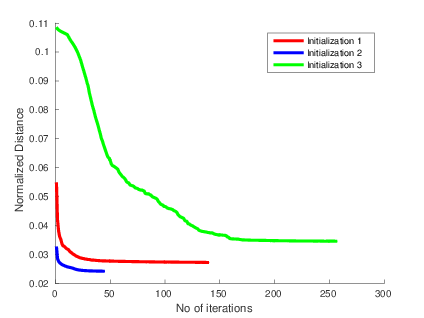
\epsfig{file=images/dist_change_euall.png,  width=0.5\textwidth}
\caption{The convergence of solution for \textbf{EUall} dataset. The number of iterations it took to converge differs for different initializations.}
\end{figure}

\begin{figure*}
\centering
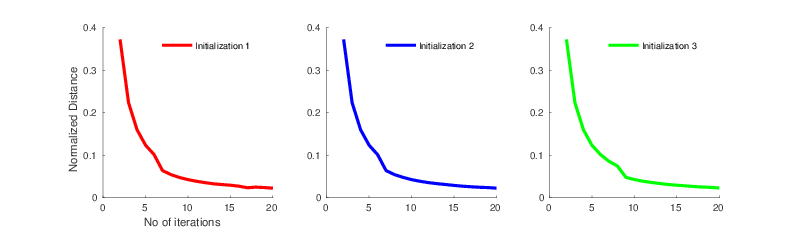
\epsfig{file=images/varying_k_distance.png,height=0.2\textheight, width=\textwidth}
\caption{The normalized distance of \textbf{facebook} dataset for different k ranging from 2 to 20.}
\end{figure*}

\begin{figure*}
\centering
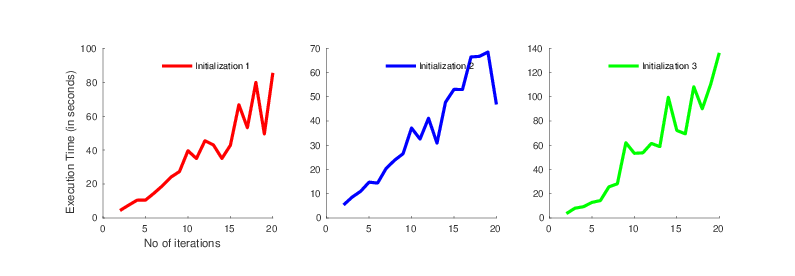
\epsfig{file=images/varying_k_time.png,height=0.2\textheight, width=\textwidth}
\caption{The execution time of \textbf{facebook} dataset for different k ranging from 2 to 20.}
\end{figure*}

\begin{figure}
\begin{tikzpicture}
\begin{axis}[xlabel={iteration $i$}, ylabel= {$\cost{\role_i} / \cost{\role'}$},
    height = 3.5cm,
    width = \columnwidth,
    cycle list name=yaf,
	yticklabel style={/pgf/number format/fixed},
	scaled ticks = false,
    %xmin = 1,
    %ymin = 0.2,
    %ymax = 1,
	ymin = 0.02,
	ytick = {0.02, 0.04, 0.06, 0.08, 0.1},
    xtick = {1, 51, 101, 151, 201, 251},
	legend entries = {\alginitrnd, \alginitdeg, \alginitone, \alginitkm}
    ]

\addplot+[no markers]
    table[x expr = {\coordindex + 1}, y index = 1, header = false]  {images/plot data/euall_init3.log};
\addplot+[no markers]
    table[x expr = {\coordindex + 1}, y index = 1, header = false]  {images/plot data/euall_init1.log};
\addplot+[no markers]
    table[x expr = {\coordindex + 1}, y index = 1, header = false]  {images/plot data/euall_init2.log};
\addplot+[no markers]
    table[x expr = {\coordindex + 1}, y index = 1, header = false]  {images/plot data/euall_init4.log};

\pgfplotsextra{\yafdrawaxis{1}{257}{0.02}{0.11}}
\end{axis}
\end{tikzpicture}
\caption{The convergence of solution for \EUall dataset. The cost of a role assignment $r_i$ at the end of $i$th iteration,
normalized by $\cost{r'}$ such that $r'(v) = 0$, for every $v$, that is, $r'$ assigns the same role to every vertex.}
\end{figure}
\fi
